\documentclass[tikz,border=6pt]{standalone}
\usepackage[utf8]{inputenc}
\usepackage[T1]{fontenc}
\usepackage{amsmath,amssymb}
\usepackage{lmodern}
\usetikzlibrary{arrows.meta,calc}

\definecolor{ink}{HTML}{1d1d1f}
\definecolor{sub}{HTML}{515154}
\definecolor{muted}{HTML}{6e6e73}
\definecolor{amberbright}{HTML}{ff9f0a}
\definecolor{blue}{HTML}{0066cc}
\definecolor{redbright}{HTML}{ff453a}

\begin{document}
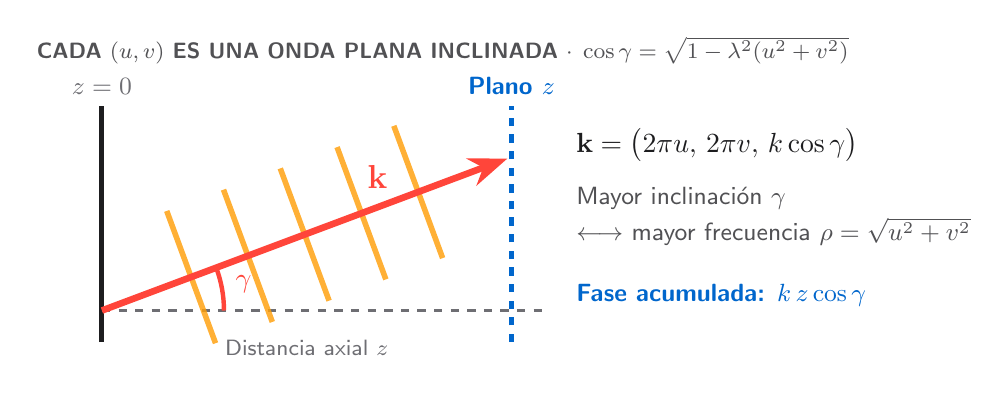
\begin{tikzpicture}[font=\sffamily,>=Stealth]

\node[anchor=west,font=\sffamily\bfseries\footnotesize,text=sub] at (0,4.55)
  {CADA $(u,v)$ ES UNA ONDA PLANA INCLINADA $\cdot\;\cos\gamma = \sqrt{1 - \lambda^2(u^2+v^2)}$};

% Planos z=0 y z
\draw[ink,line width=1.8pt] (0.95,0.85) -- (0.95,3.85);
\node[font=\sffamily\small\bfseries,text=muted] at (0.95,4.10) {$z = 0$};

\draw[blue,dashed,line width=1.8pt] (6.15,0.85) -- (6.15,3.85);
\node[font=\sffamily\small\bfseries,text=blue] at (6.15,4.10) {Plano $z$};

% Eje z horizontal
\draw[muted,dashed,line width=1.2pt] (0.95,1.25) -- (6.55,1.25);
\node[font=\sffamily\footnotesize,text=muted] at (3.55,0.78) {Distancia axial $z$};

% Frentes de onda planos exactamente perpendiculares al vector k
\coordinate (k0) at (0.95,1.25);
\coordinate (k1) at (6.10,3.18);
\foreach \t in {0.22, 0.36, 0.50, 0.64, 0.78} {
  \coordinate (C) at ($(k0)!\t!(k1)$);
  \draw[amberbright,line width=2.0pt,opacity=0.82]
    ($(C) + (-0.31, 0.84)$) -- ($(C) + (0.31, -0.84)$);
}

% Vector de onda k (encima de los frentes)
\draw[->,redbright,line width=2.4pt] (k0) -- (k1);
\node[font=\sffamily\large\bfseries,text=redbright] at (4.45,2.94) {$\mathbf{k}$};

% Ángulo gamma
\draw[redbright,line width=1.6pt] (k0) ++(0:1.55) arc (0:20.5:1.55);
\node[font=\sffamily\normalsize\bfseries,text=redbright] at (2.75,1.58) {$\gamma$};

% Leyenda derecha
\node[anchor=west,font=\sffamily\normalsize\bfseries,text=ink] at (6.85,3.35)
  {$\mathbf{k} = \bigl(2\pi u,\,2\pi v,\,k\cos\gamma\bigr)$};

\node[anchor=west,font=\sffamily\small,text=sub,align=left] at (6.85,2.45)
  {Mayor inclinación $\gamma$\\[2pt]$\longleftrightarrow$ mayor frecuencia $\rho = \sqrt{u^2+v^2}$};

\node[anchor=west,font=\sffamily\small\bfseries,text=blue] at (6.85,1.45)
  {Fase acumulada: $k\,z\cos\gamma$};

\end{tikzpicture}
\end{document}
